\subsection{Сума нерухомих точок}
Граничний розподіл суми нерухомих точок можна отримати, користуючись функціоналом Лапласа точкового процесу Пуассона.
Згідно з означенням \ref{def:poiss_proc}, для процесу Пуассона з мірою інтенсивності 
$\theta \cdot \mathrm{Leb}$ на $[0, 1]$ цей функціонал задається як
\begin{equation}\label{laplace_functional}
    \psi_N(f) = \exp\left\{ - \; \theta \int_0^1 \left(1 - e^{-f(x)}\right) \d x\right\}
\end{equation}
для вимірних, невід'ємних, обмежених функцій $f$ на $[0, 1]$.

Позначатимемо $\Sum(N)$ суму атомів точкового процесу Пуассона $N$. 
Для будь-якої точкової міри $\mu$, 
$\Sum(\mu) = \int_0^1 x \d\mu$. 
Перетворення Лапласа невід'ємної випадкової величини $X$ задається
$\L{X}(p) = \E e^{-pX}$. 
Якщо порівняти це означення з \eqref{laplace_functional}, можна побачити, що
перетворення Лапласа $\Sum(N)$ дорівнює значенню $\psi_N(f)$ для $f(x) = px$.
Пряме обчислення дає наступний результат:
\begin{gather}\label{laplace_of_sum}
    \L{\Sum(N)}(p) = 
    \exp\left\{- \theta \left( 1 + \frac{1}{p}(e^{-p} - 1)\right) \right\}.
\end{gather}

Оскільки розподіл $\Sum(N)$ є сумішшю абсолютно неперервного розподілу та
дискретного з атомом в 0, можна знайти перетворення Лапласа
лише абсолютно неперервної частини, що також буде перетворення для
$\Sum(\widehat{N})$.
\begin{gather}
    \L{\Sum(N)}(p) = \E e^{-p\cdot\Sum(N)} = 
    1 \cdot \P{\Sum(N) = 0} + \nonumber \\ +
    \E e^{-p\cdot\Sum(\widehat{N})} \cdot \P{\Sum(N) > 0} =
    e^{-\theta} + \L{\Sum(\widehat{N})}(p) \cdot (1-e^{-\theta})
    \nonumber \\
    \L{\Sum(\widehat{N})}(p) = \frac{1}{1 - e^{-\theta}}
    \left(\L{\Sum(N)}(p) - e^{-\theta}\right) = \nonumber \\ =
    \label{laplace_of_sum_cont}
    \frac{e^{-\theta}}{1 - e^{-\theta}} \cdot 
    \left(\exp\left\{- \frac{\theta}{p}(e^{-p} - 1) \right\} - 1\right)
\end{gather}

$\Sum(\widehat{N})$ є абсолютно неперервною випадковою величиною,
$\L{\Sum(\widehat{N})}(p)$ є перетворенням Лапласа для щільності, тому
перетворення Лапласа для функції розподілу $\Sum(\widehat{N})$
задається 
\begin{equation}\label{sum_cdf_laplace}
    \L{F_{\Sum(\widehat{N})}(x)}(p) = 
    \frac{e^{-\theta}}{1 - e^{-\theta}} \cdot \frac{1}{p} \cdot
    \left(\exp\left\{- \frac{\theta}{p}(e^{-p} - 1) \right\} - 1\right)
\end{equation}
Знаходження оберненого перетворення для \eqref{sum_cdf_laplace}
є доволі складним.

Розглянемо інший підхід до знаходження $F_{\Sum(N)}(x) = \P{\Sum(N) \leq x}$:
\begin{gather*}
    \P{\Sum(N) \leq x} = 
    \sum_{m=0}^{\infty} \P{\Sum(N) \leq x \mid N([0, 1]) = m} \P{N([0, 1]) = m}
    = \\ = \mathds{1}\left\{x\geq 0\right\}\cdot e^{-\theta} +
    \sum_{m=1}^{\infty} \P{\Sum(N) \leq x \mid N([0, 1]) = m} \frac{\theta^m}{m!} e^{-\theta}
\end{gather*}
Згідно з \cite{ContUnivDistr} (ст. 296), умовні розподіли 
$\P{\Sum(N) \leq x \mid N([0, 1]) = m}$
є розподілами Ірвіна-Голла --- розподілами 
суми $m$ незалежних випадкових величин з розподілом $\Unif{0, 1}$. Їх
функція розподілу має вигляд
\begin{gather*}
    F_s^{[m]} (x) = \begin{cases}
        0, & x < 0, \\
        \frac{1}{m!}\sum_{k=0}^{\floor*{x}} (-1)^k C_m^k (x-k)^m, & 0 \leq x < m, \\
        1, & x \geq m.
    \end{cases}
\end{gather*}
Для кожного інтервалу $[n, n+1)$, $n\in \N_0$, 
$\P{\Sum(N) \leq x}$  може бути виражена через $I_{\nu}(z)$, $\nu \in \R$  ---
модифіковані функції Бесселя першого роду (\cite{Abramowitz_Stegun}, ст. 375):
\begin{equation*}
    I_{\nu}(z) = \left(\frac{1}{2} z\right)^{\nu}
    \sum_{k=0}^{\infty} \frac{
        \left(\frac{1}{4} z^2 \right)^{k}
    }{
        k! \Gamma(\nu + k + 1)
    }
\end{equation*}
Отримаємо відповідну формулу. Нехай $x \in [n, n+1)$,
\begin{gather*}
    e^{\theta} \cdot \P{\Sum(N) \leq x} = 
    1 + \sum_{m=1}^{\infty} \P{\Sum(N) \leq x \mid N([0, 1]) = m} \frac{\theta^m}{m!} = \\ =
    1 + \sum_{m=1}^{n} 1 \cdot \frac{\theta^m}{m!} + 
    \sum_{m=n+1}^{\infty} \left(
        \frac{1}{m!}\sum_{k=0}^{n} (-1)^k C_m^k (x-k)^m
    \right) \frac{\theta^m}{m!} = \\ =
    \sum_{m=0}^{n} \frac{\theta^m}{m!} + 
    \sum_{m=n+1}^{\infty} \left(
        \sum_{k=0}^{n} (-1)^k \frac{1}{k! (m-k)!} (x-k)^m
    \right) \frac{\theta^m}{m!} = \\ =
    \sum_{m=0}^{n} \frac{\theta^m}{m!} + 
    \sum_{k=0}^{n} \frac{(-1)^k}{k!} \left(
        \sum_{m=n+1}^{\infty} \frac{1}{m! (m-k)!} (x - k)^m \theta^m
    \right) = \left[m - k = l \right] = \\
    = \sum_{m=0}^{n} \frac{\theta^m}{m!} + 
    \sum_{k=0}^{n} \frac{(-1)^k}{k!} \left(
        \sum_{l=n-k+1}^{\infty} \frac{1}{l! (l+k)!} (x - k)^{l+k} \theta^{l+k}
    \right) = \\ =
    \sum_{m=0}^{n} \frac{\theta^m}{m!} + 
    \sum_{k=0}^{n} \frac{(-1)^k}{k!} (x-k)^k \theta^k
    \left(
        \sum_{l=n-k+1}^{\infty} \frac{1}{l! (l+k)!} (x - k)^{l} \theta^{l}
    \right) = \\ = \left[\frac{1}{l! (l+k)!} (x - k)^{l} \theta^{l} = a_{k, l}\right] = \\ =
    \sum_{m=0}^{n} \frac{\theta^m}{m!} +
    \sum_{k=0}^{n} \frac{(-1)^k}{k!} (x-k)^k \theta^k
    \left(
        \sum_{l=0}^{\infty} a_{k, l} - 
        \sum_{l=0}^{n-k} a_{k, l} 
    \right) = \\
    = \sum_{k=0}^{n} \frac{(-1)^k}{k!}
    \left(\theta (x - k)\right)^{\frac{k}{2}} I_k\left(2\sqrt{\theta(x-k)}\right) + \\ +
    \sum_{m=0}^{n} \frac{\theta^m}{m!}
    - \sum_{k=0}^{n} \sum_{l=0}^{n-k}  \frac{(-1)^k}{k!} \frac{1}{l! (l+k)!} (x - k)^{k+l} \theta^{k+l}
\end{gather*} 
Позначимо $R(n) = \sum_{m=0}^{n} \frac{\theta^m}{m!}$,
$L(n) = \sum_{k=0}^{n} \sum_{l=0}^{n-k} \frac{(-1)^k}{k!} \frac{1}{l! (l+k)!} (x - k)^{k+l} \theta^{k+l}$.
Покажемо, що $R(n) - R(n-1) = L(n) - L(n-1)$ для всіх $n \in \N$:
\begin{gather*}
    R(n) - R(n-1) = \frac{\theta^n}{n!}, \\
    L(n) - L(n-1) = \sum_{k=0}^n \sum_{l=0}^{n-k} s_{k, l} - 
    \sum_{k=0}^{n-1} \sum_{l=0}^{n-k-1} s_{k, l} = \sum_{i=0}^n s_{i, n-i} = \\ =
    \sum_{i=0}^n \frac{(-1)^i}{i!} \frac{1}{(n-i)! n!} (x - i)^n \theta^n = 
    \frac{\theta^n}{n!} \cdot \frac{1}{n!} \sum_{i=0}^n (-1)^i C_n^i (x-i)^n.
\end{gather*}
Розглянемо функцію $f(x) = x^n$.
Ліва скінченна різниця першого порядку для $f$ з кроком $h=1$ --- це 
$\Delta f(x) = f(x) - f(x-1)$, другого порядку --- $\Delta^2 f(x) = \Delta f(x) - \Delta f(x-1) = 
f(x) - 2f(x-1) + f(x-2)$,
аналогічно рекурентно визначаються скінченні різниці вищих порядків.
Загальною формулою для різниці $k$-того порядку буде
$\Delta^k f(x) = \sum_{i=0}^k (-1)^i C_k^i f(x-i) = \sum_{i=0}^k (-1)^i C_k^i (x - i)^n$,
тому вираз $\sum_{i=0}^n (-1)^i C_n^i (x-i)^n$ --- це ліва скінченна різниця $n$-того порядку для
$x^n$. Оскільки кожна скінченна різниця є поліном порядку на 1 менше, ніж попередня,
то різниця $n$-того порядку вже буде константою. Виявляється,
що
\begin{gather*}
    \frac{1}{n!} \Delta^n f(n) = 
    \frac{1}{n!} \sum_{i=0}^n (-1)^i C_n^i (n - i)^n = 
    \frac{1}{n!} \sum_{k=0}^n (-1)^{n-k} C_n^k k^n = {n\brace n} = 1,
\end{gather*}
де ${n \brace m}$ позначає число Стірлінґа другого роду (\cite{Abramowitz_Stegun}, ст. 824-825).
Отже, $R(n) - R(n-1) = L(n) - L(n-1)$ для всіх $n \in \N$. Оскільки
$R(0) = L(0) = 1$, то $R(n) = L(n)$ для всіх $n \in \N$.
Таким чином, отримуємо 
\begin{gather}
    F_{\Sum(N)}(x) = e^{-\theta}
    \sum_{k=0}^{n} \frac{(-1)^k}{k!}
    \left(\theta (x - k)\right)^{\frac{k}{2}} I_k\left(2\sqrt{\theta(x-k)}\right), \; x \in [n, n+1).
\end{gather}
Зауважимо, що 
$F_{\Sum(N)}(0) = \left.e^{-\theta} I_0\left(2 \sqrt{\theta x}\right) \right|_{x = 0} = e^{-\theta} = \P{\Sum(N) = 0}$.

В свою чергу, функція розподілу $\Sum(\widehat{N})$ 
може бути виражена через $F_{\Sum(N)}(x)$ наступним чином:
\begin{gather}
    \P{\Sum(\widehat{N}) \leq x} = \P{\Sum(N) \leq x \mid \Sum(N) > 0} = 
    \begin{cases}
        0, & x < 0, \\
        \frac{F_{\Sum(N)}(x) - e^{-\theta}}{1-e^{-\theta}}, & x \geq 0.
    \end{cases}
\end{gather}
Оскільки $\Sum(\widehat{N})$ є абсолютно неперервною випадковою величиною, можна також знайти
її щільність розподілу. Зробимо це для $x \in [n, n+1), n \in \N_0$. Оскільки
$I_{\nu} ' (z) = I_{\nu+1} (z) + \frac{\nu}{z} I_{\nu} (z)$ (\cite{Abramowitz_Stegun}, ст. 376),
то для $z = z(x) = \sqrt{\theta(x-k)}$ і 
$g_k(x) = g_k(z(x)) = \left(\theta (x - k)\right)^{\frac{k}{2}} I_k\left(2\sqrt{\theta(x-k)}\right) = z^k I_k(2z)$
маємо
\begin{gather*}
    g_k'(x) = \left(
        k z^{k-1} I_k(2z) + 2 z^k \left(I_{k+1}(2z) + \frac{k}{2z} I_k(2z)\right)
    \right) z'(x) = \\ =
    2 z^{k-1} \left(k I_k(2z) + z I_{k+1}(2z)\right) \cdot z'(x) = 
    2 z^{k-1} \left(k I_k(2z) + z I_{k+1}(2z)\right) \cdot \frac{\theta}{2 z} = \\ =
    \theta z^{k-2} \left(k I_k(2z) + z I_{k+1}(2z)\right) = \\ =
    \theta \left(\theta (x - k)\right)^{\frac{k}{2}-1}
    \left(
        k I_k \left(2 \sqrt{\theta (x - k)} \right) + 
        \sqrt{\theta (x - k)} I_{k+1} \left(2 \sqrt{\theta (x - k)}\right)
    \right)
\end{gather*}
Таким чином, отримуємо
\begin{gather}
    f_{\Sum(\widehat{N})}(x) = \frac{e^{-\theta}}{1 - e^{-\theta}} \sum_{k=0}^{n} \frac{(-1)^k}{k!} g_k'(x), \; x \in [n, n+1).
\end{gather}

При цьому, значення $\E\Sum(N)$ значно простіше знайти
за формулою повного математичного сподівання,
оскільки для $m > 0$ $\E\left(\Sum(N) \mid N([0, 1]) = m\right) = \frac{m}{2}$
як математичне сподівання суми $m$ незалежних випадкових величин
з розподілом $\Unif{0, 1}$:
\begin{gather*}
    \E\Sum(N) = 0\cdot \P{N([0, 1]) = 0} +
    \sum_{m=1}^{\infty} \frac{m}{2} \frac{\theta^m}{m!} e^{-\theta} =
    \frac{e^{-\theta}}{2}\sum_{m=1}^{\infty} \frac{\theta^m}{(m-1)!} = \frac{\theta}{2}
\end{gather*}

Сформулюємо отриманий результат у вигляді теореми.
\begin{theorem}
    Нехай $\sigma \sim \ESF{n, \theta}$, а 
    $S_n = \sum_{i : \sigma(i) = i} i = \sum_{i=1}^n i \cdot \mathds{1}\left\{\sigma(i) = i \right\}$ --- сума нерухомих точок $\sigma$.
    Тоді при $n\to\infty$ виконується граничне
    співвідношення
    $\frac{S_n}{n} \overset{d}{\longrightarrow} S$,
    де функція розподілу випадкової величини $S$ дорівнює
    \begin{gather}
        F_{S}(x) = \begin{cases}
            0, & x < 0, \\
            e^{-\theta}
            \sum\limits_{k=0}^{\floor*{x}}
            (-1)^k \frac{1}{k!}\left(\theta(x-k)\right)^{\frac{k}{2}} I_k\left(2\sqrt{\theta(x-k)}\right), & x \geq 0,
        \end{cases}
    \end{gather}
    а її перетворення Лапласа має вигляд \eqref{laplace_of_sum}.
    
    Якщо позначити $\widehat{S}_n$ суму нерухомих точок за умови,
    що вони взагалі існують, то виконуються також граничне співвідношення
    $\frac{\widehat{S}_n}{n} \overset{d}{\longrightarrow} \widehat{S}$,
    де $\widehat{S}$ є абсолютно неперервною випадковою величиною з
    функцією та щільністю розподілу
    \begin{gather}
        F_{\widehat{S}}(x) = \begin{cases}
            0, & x < 0, \\
            \frac{F_{S}(x) - e^{-\theta}}{1 - e^{-\theta}}, & x \geq 0,
        \end{cases},\;
        f_{\widehat{S}}(x) = \begin{cases}
            0, & x < 0, \\
            \frac{\theta e^{-\theta}}{1 - e^{-\theta}}
            \sum_{k=0}^{\floor*{x}} \frac{(-1)^k}{k!} f_k(x), & x \geq 0,
        \end{cases},
    \end{gather}
    де $f_k(x)$ визначено як 
    $$f_k(x) = \left(\theta (x - k)\right)^{\frac{k}{2} - 1}
    \left(
        k I_k \left(2 \sqrt{\theta (x - k)} \right) + 
        \sqrt{\theta (x - k)} I_{k+1} \left(2 \sqrt{\theta (x - k)}\right)
    \right),$$
    а її перетворення Лапласа має вигляд \eqref{laplace_of_sum_cont}.
    \begin{figure}[H]
        \centering
        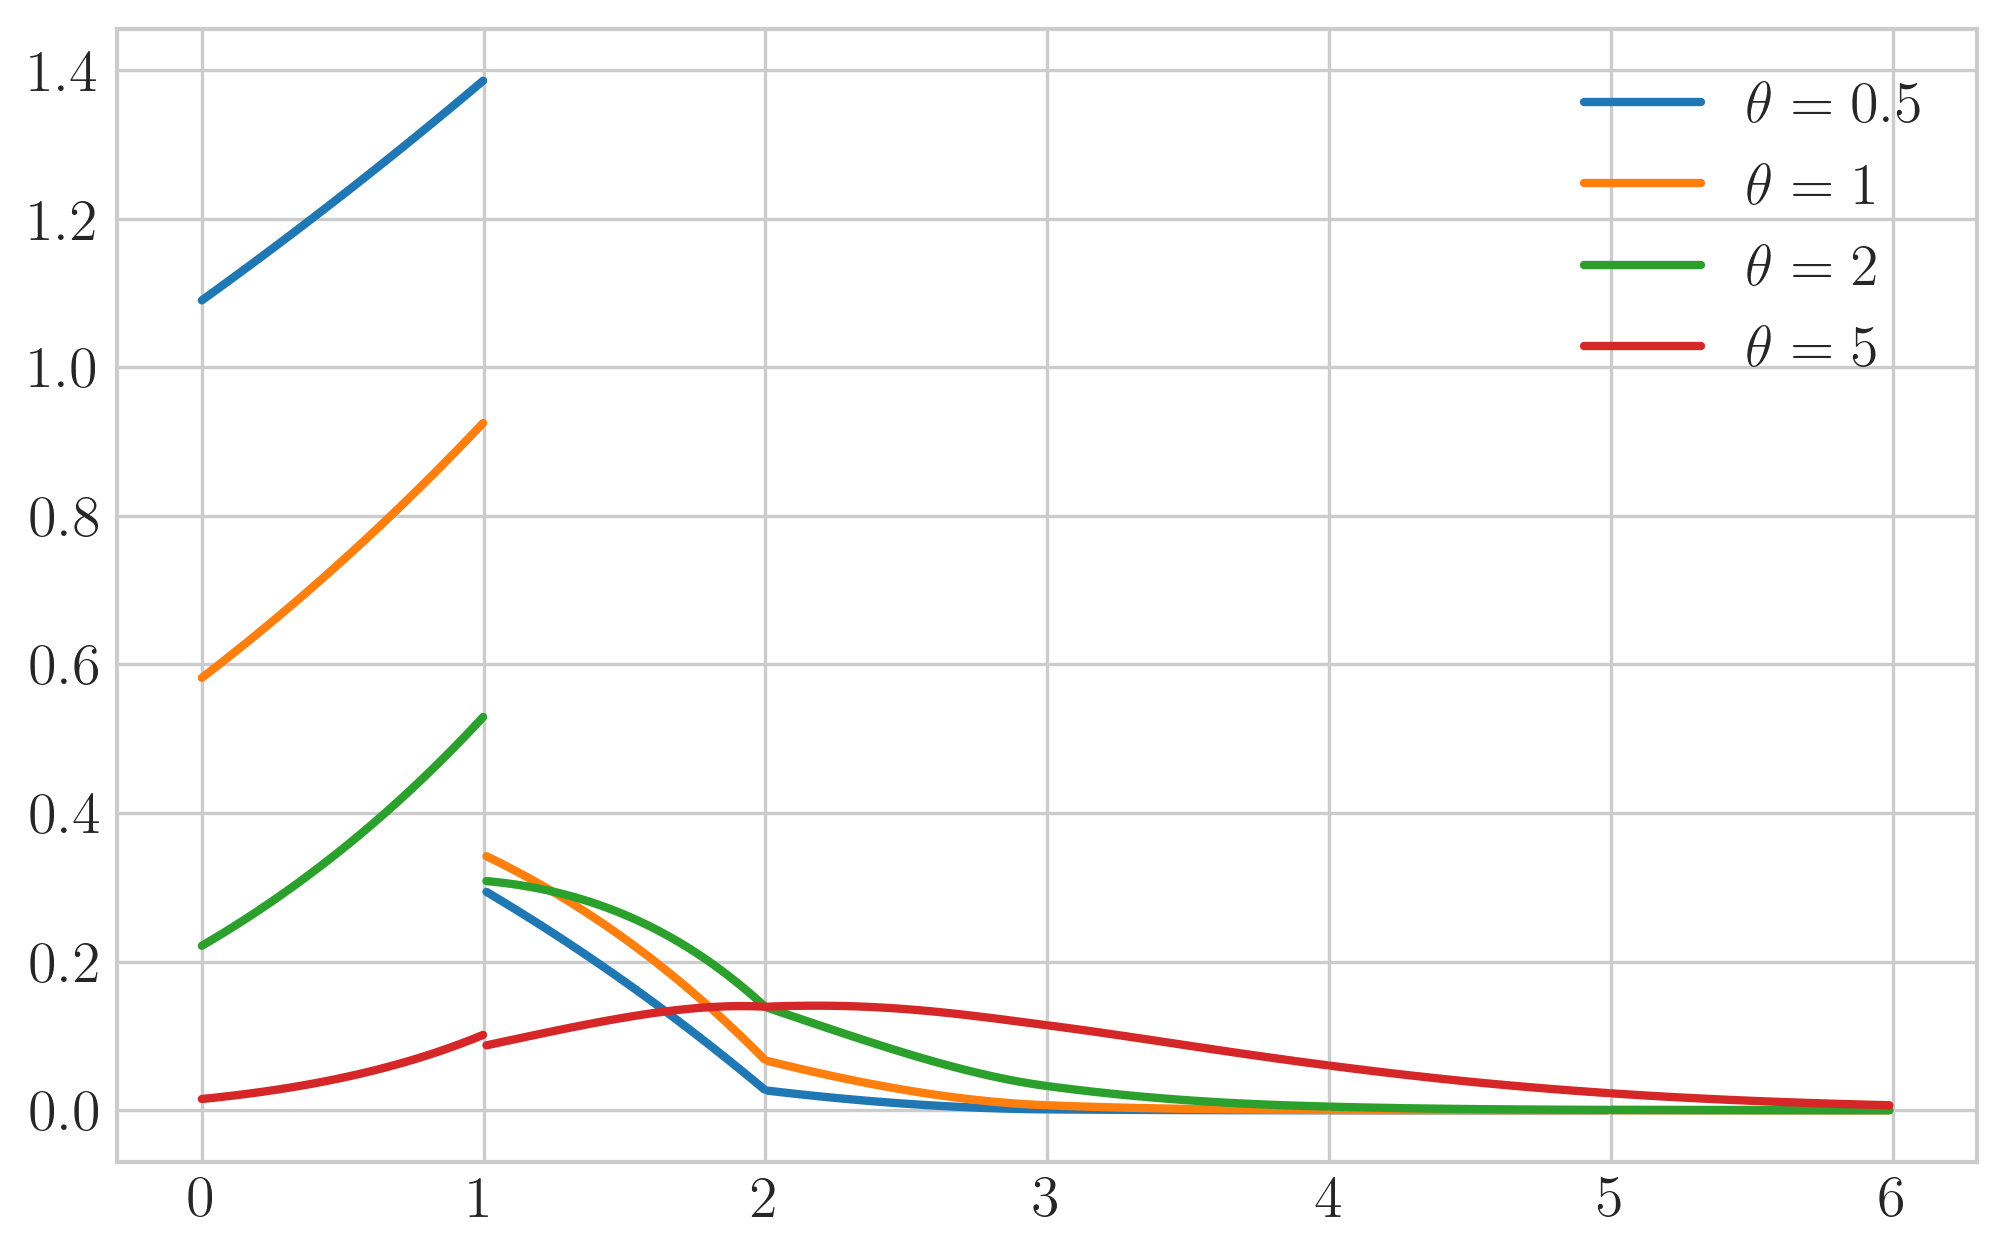
\includegraphics[scale=0.65]{plots/pdf_sum_hat.png}
        \caption{Графіки щільності розподілу $f_{\widehat{S}}(x)$ для різних значень $\theta$.}
    \end{figure}
\end{theorem}